\begin{enumerate}[label=\thesection.\arabic*.,ref=\thesection.\theenumi]
\numberwithin{equation}{enumi}

\item For an LTI system, the Bode plot for its gain defined as
\begin{align}
	G(s) = 20\log \abs{H(s)}
	\label{eq:ep18btech11016_gain}
\end{align}
is as illustrated in the Fig. \ref{fig:ep18btech11016_bode}. Find the corner frequencies $\omega_{01}$ and $\omega_{02}$ from the plot.

\begin{figure}[ht!]
\centering
    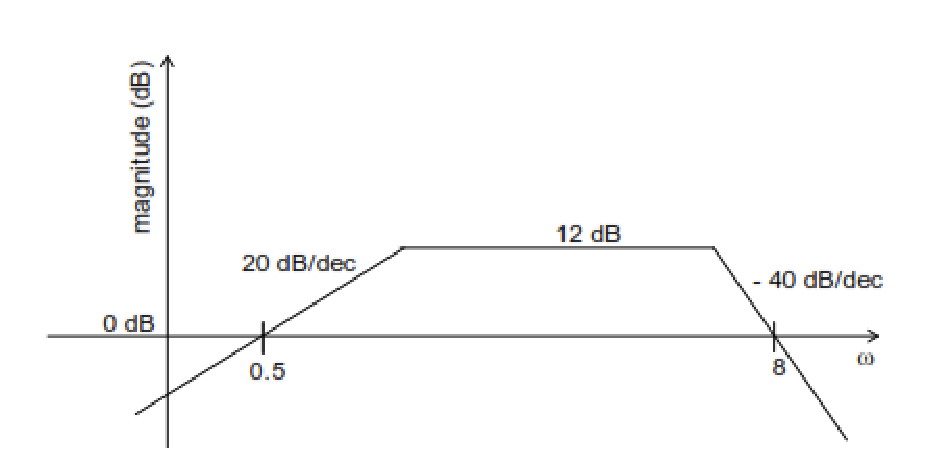
\includegraphics[width=\columnwidth]{./figs/ep18btech11016/ep18btech11016_fig1.eps}
    \caption{}
    \label{fig:ep18btech11016_bode}
\end{figure}

\solution
The corner frequencies can be calculated using 
\begin{align}
    slope &= \frac{M_2 - M_1}{\log \omega_2 - \log \omega_1}
\\
\implies    -40 &= \frac{0 - 12}{\log 8 - \log \omega_{02}} \text{ and}
\\
    20 &= \frac{0 - 12}{\log 0.5 - \log \omega_{01}}
\\
\implies     \omega_{02} = 4,    \omega_{01} = 2
\end{align}

%----------------------------------------------------------------------------%

\item Express the given bode plot as a piece-wise linear function.
\\
\solution
\begin{align}
\abs{ G\brak{\j\omega}} = 
 \begin{cases} 
        20\log 2\omega & 0 < \omega \leq 2 \\
      12 & 2 \leq \omega \leq 4 \\
      -40\log\frac{\omega}{8} & \omega \geq 4
 \end{cases}
\end{align}

%----------------------------------------------------------------------------%

\item Find the transfer function from the calculated frequencies.
\\
\solution  From Fig.     \ref{fig:ep18btech11016_bode} we observe the following

\begin{enumerate}
\item Since the initial slope is +20, there must be a zero at the origin.
\item At $\omega_{01}$, the change in slope is -20dB, so there exists one pole at this frequency.
\item At $\omega_{02}$, the change in slope is -40dB, so there exist two poles at this frequency.
\end{enumerate}
Therefore, the transfer function is,
\begin{align}
\label{eq:ep18btech11016_est_gain}
   G(s) =  \frac{Ks}{\brak{1 + \frac{s}{2}}\brak{1 + \frac{s}{4}}^2} 
\end{align}
%---------------------------------------------------------------------------%


%---------------------------------------------------------------------------%

\item Verify \eqref{eq:ep18btech11016_est_gain} by plotting the bode plot and comparing with   Fig.  \ref{fig:ep18btech11016_bode}.
\\
\solution Se Fig. \ref{fig:ep18btech11016_fig2} generated by 
\begin{lstlisting}
codes/ep18btech11016.py
\end{lstlisting}
\begin{center}
    \begin{figure}[!h]
    \centering
    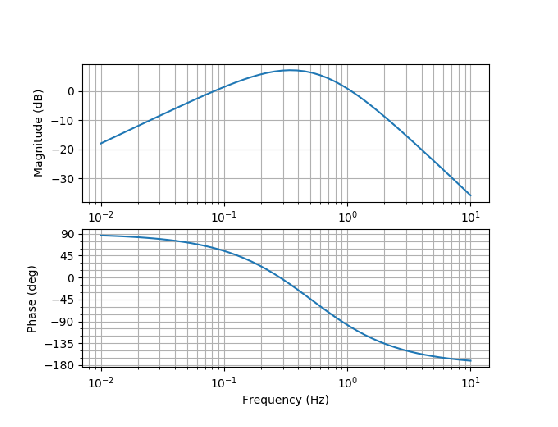
\includegraphics[width=\columnwidth]{./figs/ep18btech11016/ep18btech11016_fig2.eps}
    \caption{Plot of G(s)}
    \label{fig:ep18btech11016_fig2}
    \end{figure}
\end{center}


\end{enumerate}
